\documentclass[t]{beamer} \usepackage[czech]{babel} \usepackage[utf8]{inputenc} \usetheme{Frankfurt} %{{{
\usefonttheme{serif} \usepackage{palatino}
\let\OLDsection\section \renewcommand{\section}[1]{\OLDsection{#1} \subsection{}} % each slide has a bullet even when no subsections used
\usepackage{booktabs,amsmath,amsfonts,graphicx,sidecap}
\usepackage{tikz} \tikzstyle{every picture}+=[remember picture] \everymath{\displaystyle}
\usepackage{textpos} 

\beamersetleftmargin{3mm} \beamersetrightmargin{3mm}
\definecolor{myblue}{rgb}{0.10, 0.30, 0.50}
\usecolortheme[named=myblue]{structure}
\setbeamertemplate{navigation symbols}{\color{myblue}\footnotesize\insertframenumber}			% leave only tiny page number at the bottom
\setbeamerfont*{frametitle}{size=\normalsize,series=\bfseries}
%}}}
\hypersetup{
        pdftitle={Metamaterials for the Terahertz Spectral Range},
        pdfauthor={Ing. Filip Dominec},
        pdfsubject={},
        pdfkeywords={}
}

\title[short title]{full title}
\author{name surname} \institute{} \date{}

\begin{document}
\section{Introduction}

\begin{frame}		%{{{ Titulní stránka
	\titlepage
\end{frame}		%}}}
\section{Introduction}
%\begin{frame}[plain]{\tiny{\vspace{-1em}A text\vspace{-.5em}}}	%{{{

\begin{frame}{What are metamaterials and photonic crystals?}	%{{{

\begin{exampleblock}{Waves in periodic structures vs. in natural media}
\centering \begin{tabular}{lcccr}
Light in MMs    &$\leftrightarrow$  &$\lambda \gg a$ &$\leftrightarrow$ 	& Light in a crystal         	\\
Light in PhCs   &$\leftrightarrow$  &$\lambda \sim a$ &$\leftrightarrow$ 	& Electron wave in a crystal 	\\
\end{tabular}
\end{exampleblock}


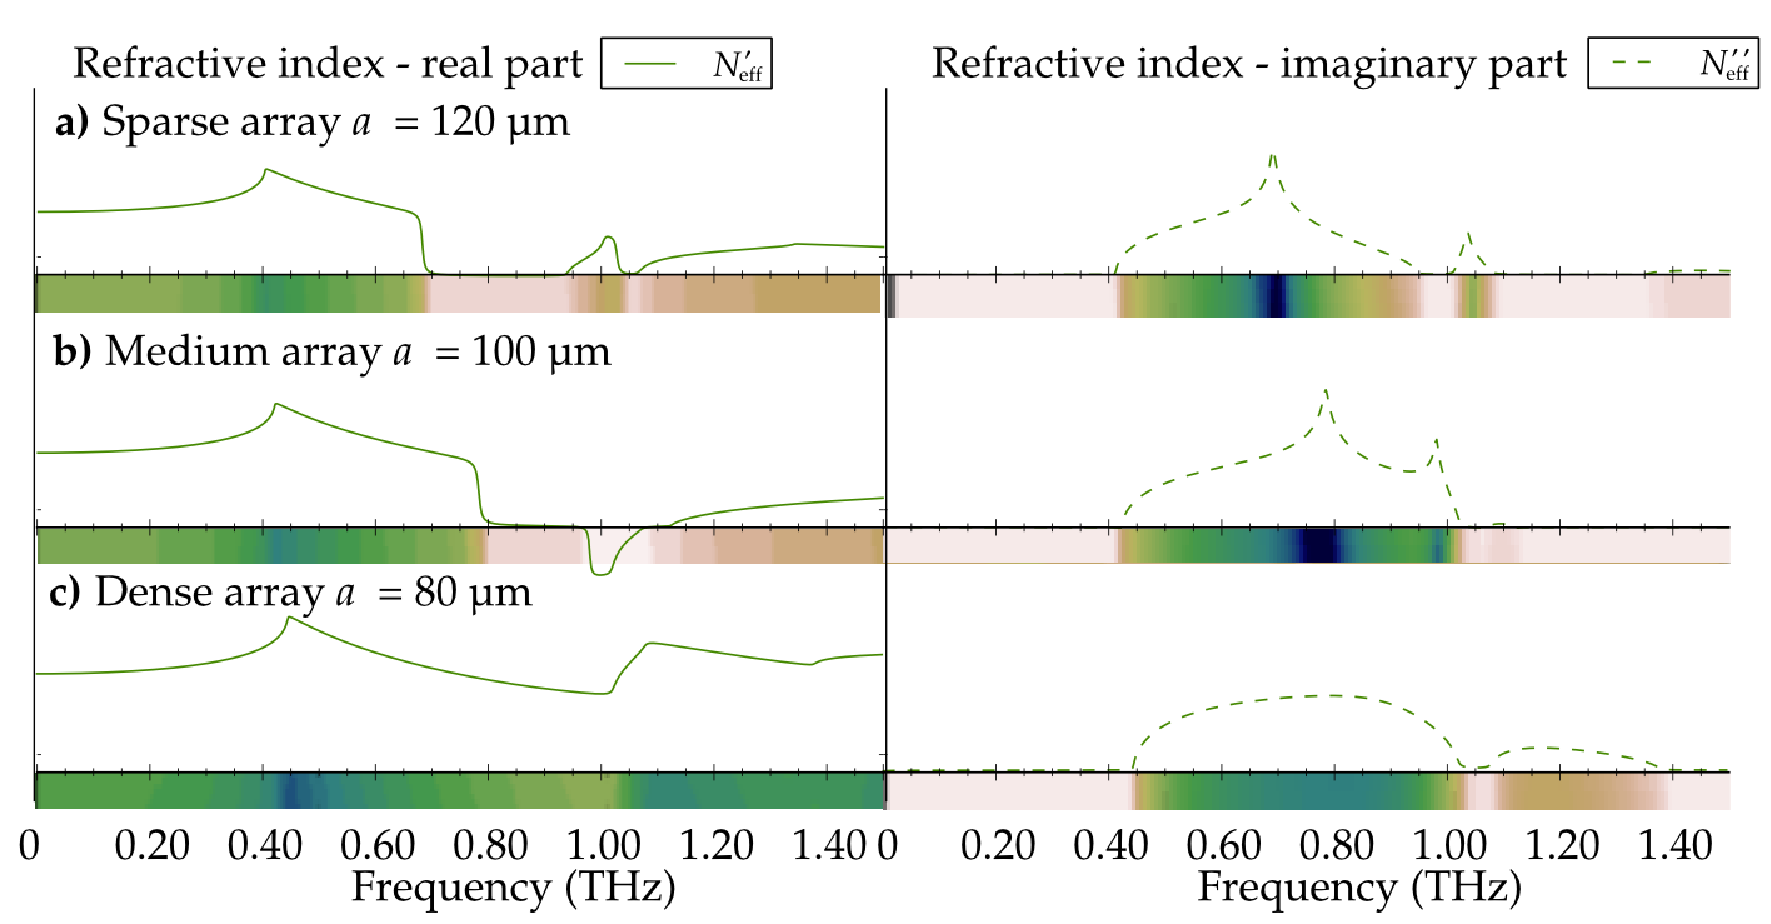
\includegraphics[width=1.\framewidth]{../img/ERods_sketch_of_separate_spectra_to_continuous_scan.pdf}

oetoeteuco uohsauo ecuhasoe uhaontehuas,c.uh sa,.huksa,nch ksa,hc ksa,hc kshca,.sk akjhc as,hkc sa,hk a
k a ks,.k a,
\end{frame} 		%}}}


\begin{frame}{Early metamaterials} 		%{{{
[figure of 1940's artificial diel] early metamaterials (known as Artificial dielectrics) used to enhance or reduce eff. permittivity 
\end{frame} 		%}}}

\begin{frame}{Early photonic crystals} 		%{{{
[figure of 1980's Yablonovite]    
Engineering of the photonic band gap (c.f. electrons in crystal)
\end{frame} 		%}}}

\begin{frame}{2000's: Merging of paradigms?} 		%}}}
Two notions, metamaterials (also known as artificial dielectrics) and photonic crystals developed separately
The fundamental difference was in the ratio of periodicity compared to the wavelength

However, as the metamaterial research approaches the optical frequencies,  the $\lambda \gg a$ limit can not be held

Note that this is determined by available materials (not a mere issue of our technology)

Since 2000s, the research is getting into the boundary region between PhCs and MMs. [citations of NIR/optical MMs] 

We must carefully review the simple approaches to MMs that assumed the unit cell $a$ to be \textit{just small}
\end{frame} 		%}}}




\begin{frame}{}	%{{{
\end{frame} 		%}}}


\begin{frame}{A figure}	%{{{

\begin{columns}[T] % align columns
\begin{column}{.5\textwidth}
\vspace{3mm}
\noindent Description text
\end{column}%
\begin{column}{.5\textwidth}
%\begin{figure}[h] \label{fg_} \centering 
%\includegraphics[width=5cm]{img/figure.pdf}
%\end{figure}
\end{column}%
\end{columns}

\end{frame} 		%}}}

\section{Section2}
\begin{frame}[fragile] \frametitle{A Python code}%{{{
\begin{scriptsize}
\end{scriptsize}
\end{frame}
%}}}

\end{document}

